\documentclass[conference]{IEEEtran}

% --- minimal packages for stand-alone figures/tables ---
\usepackage{graphicx}
\usepackage{tikz}
\usepackage{pgfplots}
\pgfplotsset{compat=1.18}
\usetikzlibrary{arrows.meta,positioning}

\begin{document}

% ===== Title (centered, a bit larger) =====
\begingroup
\centering
{\LARGE \textbf{Figures and Tables for}}\\[0.25em]
{\Large ``FeFET CMOS 0.18~$\mu$m Integration Study''}\par
\endgroup
\vspace{1.0em}

% ================= Page 1: Process Integration =================
\section*{Figures and Tables (Process Integration)}

% -------- Fig.1 (centered) --------
\begin{figure}[!t]
\centering
% ======= ここにあなたの最新版の TikZ フロー図 =======
% \begin{tikzpicture}[...]
% ...
% \end{tikzpicture}
% ============================================
\caption{Placement of the FeFET gate-last module within the 0.18~$\mu$m CMOS baseline (vertical layout).}
\end{figure}

% Fig.1 と Table I の間隔を広めに
\vspace{1.2em}

% -------- Table I (centered) --------
\begin{table}[!t]
\centering
\caption{Added masks / process steps relative to baseline logic.}
\begin{tabular}{|c|c|l|}\hline
Step & Mask & Comment\\ \hline
FE metal gate & +1 & Reuse analog option route\\
FE anneal     & 0  & Performed in BEOL furnace (no extra mask)\\ \hline
\end{tabular}
\end{table}

\clearpage % ここで 2 ページ目へ

% ================= Page 2: Reliability Data =================
\section*{Figures and Tables (Reliability Data)}

% -------- Fig.2: Endurance (centered, full width) --------
\begin{figure}[!t]
\centering
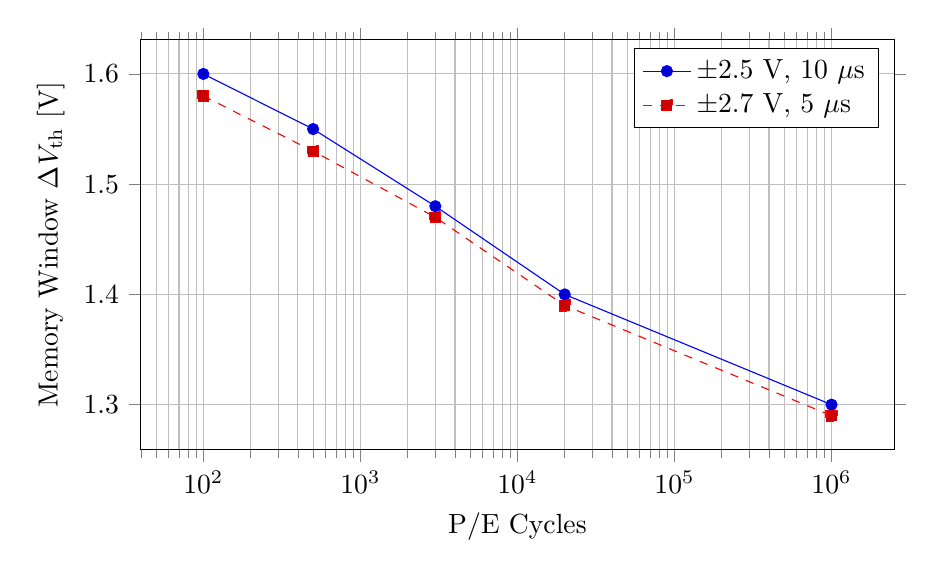
\begin{tikzpicture}
\begin{axis}[
  width=0.92\linewidth, height=0.56\linewidth,
  xlabel={P/E Cycles}, xmode=log, log basis x=10,
  ylabel={Memory Window $\Delta V_{\mathrm{th}}$ [V]},
  grid=both, tick align=outside, legend cell align=left]
\addplot+[mark=*, line join=round] coordinates {(1e2,1.60) (5e2,1.55) (3e3,1.48) (2e4,1.40) (1e6,1.30)};
\addlegendentry{$\pm 2.5$ V, 10 $\mu$s}
\addplot+[mark=square*, dashed, line join=round] coordinates {(1e2,1.58) (5e2,1.53) (3e3,1.47) (2e4,1.39) (1e6,1.29)};
\addlegendentry{$\pm 2.7$ V, 5 $\mu$s}
\end{axis}
\end{tikzpicture}
\caption{Schematic endurance behavior of HZO-FeFETs in a 0.18~$\mu$m flow.}
\end{figure}

% -------- Fig.3: Wake-up & Retention (縦並び・centered) --------
\begin{figure}[!t]
\centering
% Wake-up
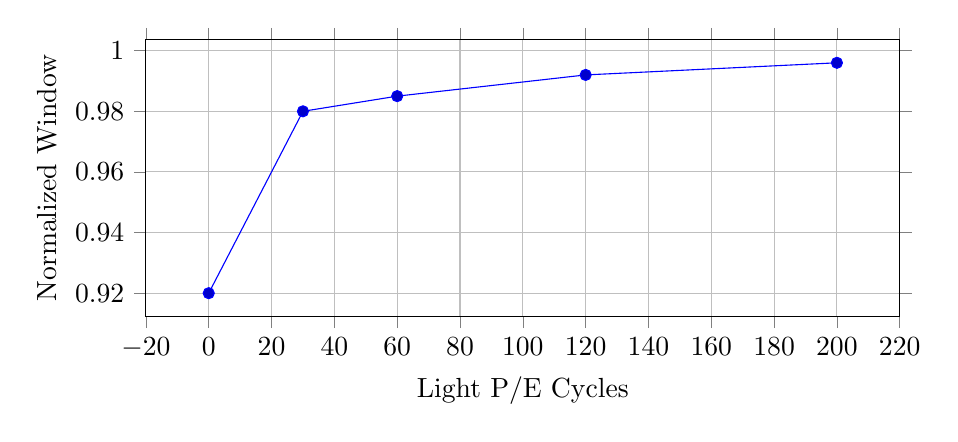
\begin{tikzpicture}
\begin{axis}[
  width=0.92\linewidth, height=0.42\linewidth,
  xlabel={Light P/E Cycles}, ylabel={Normalized Window},
  grid=both, tick align=outside]
\addplot+[mark=*, line join=round] coordinates {(0,0.92) (30,0.98) (60,0.985) (120,0.992) (200,0.996)};
\end{axis}
\end{tikzpicture}

\vspace{0.6em}

% Retention (projection)
\begin{tikzpicture}
\begin{axis}[
  width=0.92\linewidth, height=0.42\linewidth,
  xmode=log, log basis x=10,
  xlabel={Time $t$ @ 85$^\circ$C (s)},
  ylabel{$\Delta V_{\mathrm{th}}(t)/\Delta V_{\mathrm{th}}(t_0)$},
  grid=both, tick align=outside]
\addplot+[mark=*, line join=round] coordinates {(1e2,0.995) (1e3,0.985) (1e4,0.972) (1e5,0.960) (1e6,0.950)};
\end{axis}
\end{tikzpicture}
\caption{Wake-up (top) and retention projection at 85$^\circ$C (bottom).}
\end{figure}

% -------- Fig.4: TDDB Weibull (凡例を右下) --------
\begin{figure}[!t]
\centering
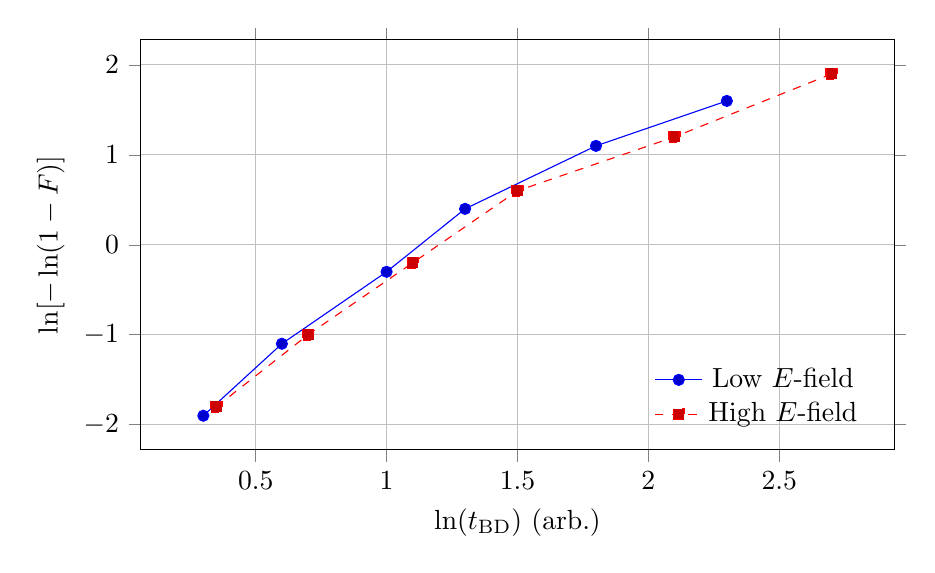
\begin{tikzpicture}
\begin{axis}[
  width=0.92\linewidth, height=0.56\linewidth,
  xlabel={$\ln(t_{\mathrm{BD}})$ (arb.)},
  ylabel={$\ln[-\ln(1-F)]$},
  grid=both, tick align=outside,
  legend style={at={(0.97,0.03)},anchor=south east, draw=none, fill=none}
]
\addplot+[mark=*, line join=round] coordinates {(0.30,-1.90) (0.60,-1.10) (1.00,-0.30) (1.30,0.40) (1.80,1.10) (2.30,1.60)};
\addlegendentry{Low $E$-field}
\addplot+[mark=square*, dashed, line join=round] coordinates {(0.35,-1.80) (0.70,-1.00) (1.10,-0.20) (1.50,0.60) (2.10,1.20) (2.70,1.90)};
\addlegendentry{High $E$-field}
\end{axis}
\end{tikzpicture}
\caption{TDDB Weibull representation at two stress fields (illustrative).}
\end{figure}

\end{document}
